%%
%% Template article for Elsevier's document class `elsarticle'
%% with harvard style bibliographic references
%%

\documentclass[preprint,12pt,authoryear]{elsarticle}

%% The amssymb package provides various useful mathematical symbols
\usepackage{amssymb}
%% The amsmath package provides equation environment
\usepackage{amsmath}
%% The algorithms
\usepackage{algorithm}
\usepackage{algorithmic}
%% The images
\usepackage{graphicx}
%% Booktabs for professional tables
\usepackage{booktabs}
%% Verbatim with URL-sensitive line breaks.
\usepackage{url}
%% Render ~ in URLs as a full-size tilde on the math axis.
\makeatletter
\def\UrlTildeSpecial{\do\~{\hbox{\m@th$\sim$}}}
\let\Url@force@Tilde\UrlTildeSpecial
\makeatother
% upright sub-index
\newcommand{\ui}[2]{#1 _{\text{#2}}}
% upright sub-index with variable
\newcommand{\uis}[3]{#1 _{\text{#2}, #3}}

%% The lineno package adds line numbers.
\usepackage{lineno}

\journal{Expert Systems with Applications}

\begin{document}

\begin{frontmatter}

    \title{From Detection to Maintenance Action: Streaming Sensor-Fault Typing for Self-Supervised Anomaly Detection in Industrial Systems}

    \author[aff1]{Marek Wadinger\corref{cor1}}
    \ead{marek.wadinger@stuba.sk}
    \cortext[cor1]{\textit{Phone numbers:} +421 902 810 324 (Marek Wadinger)}
    \ead[url]{uiam.sk/~wadinger}

    \author[aff1]{Michal Kvasnica}
    \ead{michal.kvasnica@stuba.sk}

    \affiliation[aff1]{organization={Institute of Information Engineering, Automation and Mathematics, Slovak University of Technology in Bratislava},
        addressline={Radlinskeho 9},
        postcode={812 37},
        state={Bratislava},
        country={Slovakia}
    }

    \begin{abstract}
        Streaming anomaly detectors tell operators \emph{that} a sensor reading is abnormal and, when interpretable, \emph{which} signal and in \emph{which} direction. They do not tell operators \emph{what to do}: whether to recalibrate, replace, or clean a sensor, or to investigate the process itself. We close this gap with a streaming sensor-fault classifier that attributes each flagged signal to a maintenance-relevant fault type---bias, drift, accuracy loss, or freezing---directly from the conditional residuals of a self-supervised online detector, using O(1) memory and no history buffers. On real battery-depletion faults in the Intel Berkeley Lab deployment, the composed system reaches 90\% real-fault detection at a 7.4\% healthy false-positive rate, and types the resulting faults predominantly as freezing (0.93), the signature of sensors stuck at degraded values. We further characterize the operating envelope on controlled injections: freezing and drift are recovered with recall 1.000 and 0.741, while bias recall is monotone in conditional standard deviation---the interpretable conditional model absorbs constant offsets on strongly coupled signals (recall 0.059) and isolates them on weakly coupled ones (0.941). We show that two original claims do not survive validation: freezing is not a detection blind spot of the base detector (it catches every injected freeze, usually faster than the dedicated test), and adaptation robustness comes from graded change-point suppression rather than residual cancellation. The result is a deployable typing layer with a rigorously mapped---rather than overstated---operating envelope.

    \end{abstract}

    %%Research highlights
    \begin{highlights}
        \item Streaming detector attributes each flagged sensor to a maintenance-relevant fault type
        \item Reaches 90\% real-fault detection at 7.4\% healthy false-positive rate on battery-depletion faults
        \item O(1)-memory conditional-residual typing composed with a self-supervised online detector
        \item Operating envelope characterized: bias absorption, dead-band, and correlation limits made explicit
        \item Online adaptation is mandatory; a static prefix model false-alarms at 0.97 on a diurnal stream
    \end{highlights}

    \begin{keyword}
        Fault diagnosis \sep Sensor fault classification \sep Online learning \sep Anomaly detection \sep Self-supervised learning \sep Streaming algorithms
    \end{keyword}

\end{frontmatter}

\linenumbers

\section{Introduction}
\label{Introduction}
In industrial monitoring, the cost of a sensor fault is paid not when it is detected but when it is acted upon. A reading that drifts away from its true value, a transmitter stuck at its last sample, or an instrument whose noise floor has grown all demand different maintenance responses: recalibration, replacement, cleaning, or process investigation. An operator who learns only that a signal is anomalous, and even which signal and in which direction, must still diagnose the failure mode before dispatching the correct action. The fault \emph{type} is what drives the maintenance action, and it is precisely what most streaming detectors leave to human triage.

The base detector we extend is a self-supervised, online anomaly detector for SCADA-based industrial systems~\citep{Wadinger2023}. It scores each signal by the conditional cumulative probability of its current value given the remaining signals, flags a value when that probability falls below $\alpha$ or above $1-\alpha$ (with $\alpha \approx 0.00133$, i.e.\ roughly three conditional standard deviations), and adapts its conditional model online with change-point awareness. Crucially, it is interpretable: it isolates the responsible signal and the direction of the excursion, and exposes per-signal operating limits. What it does not provide is the fault \emph{type}---it localizes the anomaly but does not characterize the failure mode, leaving the detection-to-action gap open.

We close that gap with a streaming sensor-fault classifier that attributes each flagged signal to one of four maintenance-relevant types---bias, drift, accuracy loss, or freezing---computed from the same conditional residuals the base detector already produces. The classifier maintains only a small set of exponentially weighted running statistics per signal: it uses O(1) memory, keeps no history buffers, and adds negligible cost to the streaming pipeline. The fault taxonomy itself is not new; we adopt the bias / noise / constant / drift categories established for sensor faults in wireless and environmental sensing~\citep{Sharma2010,Ni2009}. Our contribution is the \emph{streaming conditional-residual realization} of this taxonomy, composed directly with a self-supervised detector so that type attribution rides on the same online statistics as detection.

We lead with the practical outcome. On real battery-depletion faults from the Intel Berkeley Lab deployment~\citep{IntelLab2004}---where a mote's failing battery degrades its temperature and humidity readings to physically impossible values---the composed system reaches 90\% real-fault detection at a 7.4\% healthy false-positive rate, and types the resulting faults predominantly as freezing (0.93), the expected signature of a transmitter stuck at a degraded value. Online adaptation is not optional here: a static model fit on a short prefix of the same diurnal stream false-alarms at a rate of 0.97. The typing layer thus converts an adaptive detector's alarm into an actionable maintenance label on a real fault population.

We then characterize the operating envelope honestly, treating it as support for---not a qualification of---the practical result. Two claims we initially expected to hold do not survive our own validation, and we report them as refuted. First, freezing is \emph{not} a detection blind spot of the base detector: it catches every injected freeze on every channel, usually faster than a dedicated fixed-window freeze test, so the freeze test contributes type \emph{attribution} (a stuck sensor versus a process excursion), not detection capability. Second, the robustness of the adaptive detector to faults that arrive during adaptation comes from graded change-point suppression, not from conditional-residual cancellation. We treat this honesty as a feature: the envelope is mapped rather than overstated, and the limitations---bias absorption on strongly coupled signals, the limited cancellation of a two-signal conditional model, and the masking dead-band introduced by suppression---are quantified and explained.

The contributions of this paper are:
\begin{enumerate}
    \item A streaming, O(1)-memory sensor-fault classifier that types each flagged signal as normal, bias, drift, accuracy loss, or freezing from the conditional residuals of a self-supervised online detector, with no history buffers (Section~\ref{Method}).
    \item A demonstration on real battery-depletion faults that the composed system reaches 90\% real-fault detection at a 7.4\% healthy false-positive rate and assigns maintenance-relevant types, with online adaptation shown to be mandatory (Section~\ref{Results}).
    \item A rigorous characterization of the operating envelope on controlled injections, including the monotone dependence of bias recall on conditional coupling, and two refuted claims (freezing as a blind spot; residual cancellation as the source of adaptation robustness) reported as such (Sections~\ref{Results} and~\ref{Discussion}).
\end{enumerate}


\section{Related Work}
\label{Related Work}
\subsection{The base detector}
The detector we extend scores anomalies in SCADA-based industrial systems by self-supervised online learning~\citep{Wadinger2023}. For each signal it evaluates the conditional cumulative distribution of the current value given the remaining signals under a multivariate Gaussian model, flags the value when this probability lies outside $[\alpha, 1-\alpha]$ with $\alpha \approx 0.00133$, and updates the conditional model online while remaining aware of change points so that legitimate regime shifts are absorbed rather than alarmed. The detector is interpretable: it identifies the responsible signal, the direction of the excursion, and exposes per-signal operating limits. It localizes anomalies but does not classify the failure mode, which is the gap this work addresses. We reuse its conditional-residual stream as the substrate for typing rather than introducing a separate diagnostic pipeline.

\subsection{Sensor-fault taxonomies}
The categories we attribute---bias, drift, accuracy loss (noise), and freezing (constant)---are standard in the sensor-fault literature rather than novel to this work. \citet{Sharma2010} characterize the recurrent fault signatures of deployed sensors, including offset (bias), gain, and stuck-at faults, and study detection methods against them. \citet{Ni2009} likewise organize sensor data faults into a taxonomy spanning calibration offset, drift, and constant (frozen) readings. We adopt this established taxonomy unchanged; our contribution is its streaming, conditional-residual realization, not the categories themselves.

\subsection{Fault-injection protocols}
Because no public stream simultaneously labels all four fault types per signal and per timestep, controlled injection is the established route to per-type evaluation. \citet{Lai2021} introduce a benchmark methodology that injects parameterized anomaly patterns into time series to evaluate detectors under known ground truth. We follow this precedent, injecting the four typed faults into a multivariate process at controlled magnitudes and onsets so that recall and confusion can be measured per type, and we triangulate the synthetic findings against the real-fault deployment described in Section~\ref{Experimental Setup}.

\subsection{Offline fault classifiers}
A large body of work classifies sensor and process faults offline, typically by training supervised or windowed models on labelled fault episodes and extracting features over batches of history. Such methods can exploit rich temporal context but require stored windows, labelled fault data, and a training phase, which conflicts with the streaming, self-supervised, and label-free setting of the base detector. Our classifier instead derives the type from the running conditional residuals already maintained by the detector, in O(1) memory and without history buffers, so that typing is available at the same latency and operational footprint as detection.


\section{Method}
\label{Method}
\subsection{Conditional residuals as the typing substrate}
The base detector~\citep{Wadinger2023} maintains, for each signal $i$, a conditional model of its current value $x_i$ given the remaining signals $x_{-i}$. We define the conditional residual
\begin{equation}
    r_i = x_i - \uis{\mu}{cond}{i}(x_{-i}),
\end{equation}
the difference between the observed value and its conditional mean, and the conditional standard deviation $\uis{\sigma}{cond}{i}$ already used by the detector to form its score. Both quantities are available at every step at no additional modelling cost. For brevity we write $\sigma$ for the per-channel conditional standard deviation $\uis{\sigma}{cond}{i}$ in the results, and we also use $\sigma$ as a \emph{magnitude unit}---a fault or shift ``of $k\sigma$'' means $k$ multiples of the relevant conditional standard deviation; the intended sense is clear from context. The classifier operates entirely on the stream of residuals $\{r_i\}$ and their conditional scale $\uis{\sigma}{cond}{i}$: it never stores past samples and never refits a model over a window. This keeps the per-signal state to a fixed set of scalars and the per-step cost constant, matching the streaming, O(1)-memory footprint of the detector it extends.

\subsection{Running statistics}
For each signal the classifier maintains a small set of exponentially weighted moving (EWM) statistics over the residual stream. We track a fast (short half-life) and a slow (long half-life) EWM mean of $r_i$, denoted $\uis{m}{fast}{i}$ and $\uis{m}{slow}{i}$, and an EWM variance $\uis{v}{}{i}$ of $r_i$. We additionally track the EWM variance of the raw signal increments to detect a stalled transmitter. All updates are the standard constant-memory recursions; no buffer of past values is required. The half-lives are the only temporal hyperparameters of the typing layer and are shared across signals unless per-signal calibration is applied (Section~\ref{Discussion}).

\subsection{The four type tests}
Given the running statistics, a flagged signal is attributed to a type by the following tests, each expressed in units of the conditional scale so that thresholds are dimensionless.

\paragraph{Bias.} A persistent offset of the residual from zero, with stable variance, indicates a constant calibration error. We declare \emph{bias} when the slow residual mean is large in conditional-scale units, $|\uis{m}{slow}{i}| / \uis{\sigma}{cond}{i}$ exceeding a threshold, while the residual variance remains close to its baseline.

\paragraph{Drift.} A gradually growing offset is distinguished from a static one by the \emph{gap between the short- and long-horizon EWM means}. We declare \emph{drift} when $|\uis{m}{fast}{i} - \uis{m}{slow}{i}| / \uis{\sigma}{cond}{i}$ exceeds a threshold, i.e.\ when the recent residual mean is moving away from its longer-run value. We name this honestly: it is a short-versus-long EWM mean-gap statistic, \emph{not} a fitted regression slope. It requires no stored window and no least-squares fit; it responds to the direction and recency of residual movement rather than estimating a rate.

\paragraph{Accuracy loss.} An inflated noise floor with an unchanged mean indicates degraded measurement accuracy. We declare \emph{accuracy loss} when the residual variance $\uis{v}{}{i}$ exceeds its baseline by a multiplicative factor while the slow residual mean stays near zero.

\paragraph{Freezing.} A transmitter stuck at its last value produces near-zero signal increments while the conditional expectation continues to move. We declare \emph{freezing} when the EWM variance of the raw increments collapses below an absolute floor $\texttt{freeze\_eps}$ and below a fraction $\texttt{freeze\_var\_ratio}$ of the signal's marginal variance, scaled by $\texttt{freeze\_abs\_scale}$. These three constants govern how aggressively a quiet signal is judged frozen; their calibration is examined in Section~\ref{Results} (the freeze-on-quiescent ablation). A signal that satisfies none of the tests while flagged is labelled \emph{normal} with respect to typing (e.g.\ a peer signal pulled by cross-talk), and an unflagged signal is \emph{normal} by default.

\subsection{Change-point graded suppression}
A fault that arrives while the base detector is adapting to a genuine regime shift can be either masked by the adaptation or mistaken for one. The detector's change-point machinery applies a graded suppression to the typing decision around detected change points, controlled by a scale parameter \texttt{suppress\_scale}: at \texttt{scale}~$=1$ no suppression is applied, the default \texttt{scale}~$=5$ applies graded suppression, and \texttt{scale}~$=\infty$ suppresses any typing within the change-point window entirely. This parameter trades off two failure modes that we quantify separately in Section~\ref{Results}: spurious type labels from coordinated shifts in weakly correlated signals (reduced by stronger suppression) against a masking dead-band for genuine faults co-occurring with a change point (widened by stronger suppression). We treat \texttt{suppress\_scale} as the principal tuning knob of the composed system and report its effect rather than fixing it silently.


\section{Experimental Setup}
\label{Experimental Setup}
We evaluate the composed system along two complementary axes: controlled fault injection, which provides per-type ground truth, and a real fault deployment, which provides an external validity check. Because no public stream simultaneously labels all four fault types per signal and per timestep, neither axis alone suffices, and we triangulate the two. All evaluation artifacts referenced below are committed as CSV files under \texttt{examples/benchmarks/}.

\subsection{Controlled fault injection}
Following the injection-protocol precedent of~\citet{Lai2021}, we inject parameterized faults of each type---bias, drift, accuracy loss, and freezing---into a multivariate process with known ground truth, drawn from the Controlled Anomalies Time Series (CATS) benchmark~\citep{CATS2023}. Each typed fault is injected at controlled magnitude and onset onto a target signal, and recall is measured per type. We run $N=85$ trials per type in the scaled controlled validation, and report Wilson 95\% confidence intervals on every recall and precision estimate (\texttt{i7\_scaled\_per\_type.csv}). To probe the dependence of bias recall on conditional coupling, we report bias recall per target channel against that channel's conditional standard deviation (\texttt{i7\_scaled\_bias\_by\_channel.csv}, $N=17$ per channel). Freeze attribution versus base detection is evaluated on the same channels, recording per-channel freeze and CDF detection rates and detection delays (\texttt{i7\_freeze\_latency.csv}).

\subsection{Synthetic correlation control}
To separate the two robustness mechanisms of the composed system, we generate synthetic multivariate streams with controlled pairwise correlation $\rho \in \{0.1, 0.3, 0.5, 0.7, 0.9\}$ and inject coordinated shifts of magnitude $\{3, 6, 10\}$ conditional standard deviations co-occurring with a change point. For each cell we sweep the suppression scale $\texttt{suppress\_scale} \in \{1, 5, \infty\}$ (abbreviated \texttt{scale} hereafter) and report the mean false-label rate over $5$ seeds (\texttt{i7\_regime\_fp.csv}). The co-occurring-fault dead-band is measured by injecting a drift simultaneously with a change point and recording the detection magnitude at each suppression scale (\texttt{i7\_deadband.csv}). The freeze-on-quiescent ablation injects no fault into a genuinely live but quiet signal (noise floor as a fraction of marginal standard deviation) and measures the false freeze-label rate under default, strict, and loose freeze constants (\texttt{i7\_freeze\_quiescent.csv}).

\subsection{Real fault deployment}
For external validity we use the Intel Berkeley Lab sensor deployment~\citep{IntelLab2004}, in which motes report temperature and humidity over a diurnal cycle. As a mote's battery depletes (voltage below $2.3$\,V, held out as a physical fault label), its temperature and humidity readings degrade to physically impossible values---temperatures of $100$--$122$\,$^{\circ}$C and negative humidity. We treat the battery-voltage label as ground truth for a real fault, never exposing it to the detector or classifier. We sweep the detector's mean-threshold operating point and report, pooled over motes, the healthy false-positive rate and the real-fault detection rate ($N_\mathrm{healthy} \approx 1.52$M, $N_\mathrm{fault} \approx 0.39$M; \texttt{i7\_intel\_lab\_operating\_points.csv}), together with the distribution of types assigned to detected real faults (\texttt{i7\_intel\_lab\_fault\_types.csv}). To establish that online adaptation is required rather than optional, we additionally fit a static model on a short prefix of the same stream and measure its false-alarm rate.

As a second, complementary real-fault check that isolates a single labelled type, we use the LBNL building-FDD MZVAV-1 dataset~\citep{LBNL_FDD2019,Granderson2023}, an outdoor-air-temperature sensor-bias set in which a constant $\pm 1/2/4\,^\circ$C offset is imposed on the outdoor-air-temperature reading of a simulated air-handling unit over labelled date windows, with a per-timestamp fault label. We run the detector over the four coupled AHU air temperatures and report, over a mean-threshold sweep, the bias-typing recall on the biased signal against the healthy false-positive rate, together with the imposed bias magnitude in conditional-standard-deviation units (\texttt{i7\_lbnl\_bias.csv}).

\subsection{Metrics}
For the controlled injections we report per-type recall (fraction of injected faults of a type that are detected) and cross-talk precision on normal peer signals. For the real deployment we report the healthy false-positive rate and the real-fault detection rate at each operating point. All proportions estimated from finite samples are reported with Wilson 95\% confidence intervals. We do not report aggregate accuracy across types, because the type populations are not equiprobable in either the injection design or the real stream, and an aggregate would obscure the per-type and per-coupling structure that is the substance of our characterization.


\section{Results}
\label{Results}
\subsection{Real-fault operating curve}
\label{sec:operating-curve}
On the Intel Berkeley Lab deployment, the composed system detects real battery-depletion faults at a high rate while keeping healthy false alarms low, and the operator can trade the two by moving a single mean-threshold operating point. Table~\ref{tab:operating} reports the pooled sweep over motes ($N_\mathrm{healthy} \approx 1.52$M healthy samples, $N_\mathrm{fault} \approx 0.39$M fault samples; \texttt{i7\_intel\_lab\_operating\_points.csv}). At a mean threshold of $8.0$ the system reaches a $7.4\%$ healthy false-positive rate at $90.1\%$ real-fault detection; lowering the threshold to $3.0$ raises detection to $92.6\%$ at the cost of a $22.1\%$ false-positive rate. The detection rate is remarkably flat across the sweep (from $0.926$ down to $0.901$), so the operating point is chosen almost entirely by the tolerable false-alarm budget.

\begin{table}[t]
    \centering
    \caption{Real battery-depletion fault detection on the Intel Berkeley Lab deployment, online adaptive detector, pooled over motes. Source: \texttt{i7\_intel\_lab\_operating\_points.csv} ($N_\mathrm{healthy}=1\,518\,828$, $N_\mathrm{fault}=387\,671$).}
    \label{tab:operating}
    \begin{tabular}{rcc}
        \toprule
        Mean threshold & Healthy FP rate & Real-fault detection \\
        \midrule
        3.0 & 0.221 & 0.926 \\
        4.0 & 0.165 & 0.916 \\
        5.0 & 0.129 & 0.910 \\
        6.0 & 0.104 & 0.906 \\
        8.0 & 0.074 & 0.901 \\
        \bottomrule
    \end{tabular}
\end{table}

\begin{figure}[t]
    \centering
    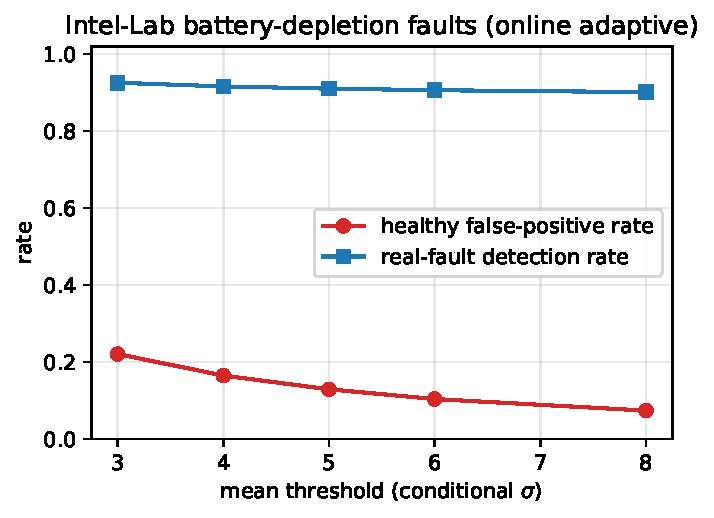
\includegraphics[width=0.8\linewidth]{figures/fig_operating_curve.pdf}
    \caption{Operating curve on the Intel Berkeley Lab battery-depletion faults (online adaptive detector, pooled over motes). Raising the mean threshold trades a lower healthy false-positive rate against a marginal drop in real-fault detection. Source: \texttt{i7\_intel\_lab\_operating\_points.csv}.}
    \label{fig:operating}
\end{figure}

Online adaptation is mandatory on this stream, not a convenience. A static model fit on a short prefix of the same diurnal signal false-alarms at a rate of $0.97$: the daily temperature and humidity cycle alone is enough to push a fixed model permanently out of distribution. The adaptive detector tracks the diurnal baseline and reserves its alarms for the battery-depletion excursions.

The types assigned to the detected real faults are dominated by freezing, as a stuck-at-degraded-value failure should be. Table~\ref{tab:realtypes} reports the type distribution over detected real-fault samples (\texttt{i7\_intel\_lab\_fault\_types.csv}): $93.2\%$ are typed freezing, $5.1\%$ drift, $1.7\%$ bias, and $0.06\%$ accuracy loss. The freezing label corresponds to the physical reality of a transmitter pinned at a corrupted reading as its battery fails, so the typing layer converts the detector's alarm into the maintenance-relevant diagnosis ``replace the mote'' rather than ``investigate the process.''

\begin{table}[t]
    \centering
    \caption{Fault types assigned to detected real faults on the Intel Berkeley Lab deployment. Source: \texttt{i7\_intel\_lab\_fault\_types.csv}.}
    \label{tab:realtypes}
    \begin{tabular}{lrr}
        \toprule
        Assigned type & Count & Fraction \\
        \midrule
        freezing      & 578\,721 & 0.932 \\
        drift         & 31\,727  & 0.051 \\
        bias          & 10\,395  & 0.017 \\
        accuracy loss & 343      & 0.001 \\
        \bottomrule
    \end{tabular}
\end{table}

The residual healthy false positives are themselves informative. Approximately $93\%$ of healthy false positives are typed as drift, arising from the healthy diurnal ramps that the two-signal conditional model (temperature given humidity, and vice versa) cannot fully cancel. This is an honest limitation tied directly to the correlation-dependence we characterize in Section~\ref{sec:regime}: with only two correlated signals available, slow shared ramps leak into the residual; a deployment with more correlated signals would suppress them further.

\subsection{Per-type recall and the bias--coupling relationship}
\label{sec:per-type}
On the scaled controlled injections, the four types are recovered at sharply different rates. Table~\ref{tab:pertype} reports per-type recall with Wilson 95\% confidence intervals over $N=85$ trials per type (\texttt{i7\_scaled\_per\_type.csv}). Freezing is recovered perfectly ($1.000$, CI $0.957$--$1.000$) and drift well ($0.741$), while accuracy loss ($0.659$) and especially bias ($0.518$) are lower. Cross-talk precision on normal peer signals is high: of the signals labelled by typing, the normal-peer label is correct with precision $\approx 0.91$ (\texttt{i7\_scaled\_normal\_precision.csv}), so coupled peers are rarely misattributed a fault.

\begin{table}[t]
    \centering
    \caption{Per-type recall on scaled controlled injections, $N=85$ trials per type, Wilson 95\% CI. Source: \texttt{i7\_scaled\_per\_type.csv}.}
    \label{tab:pertype}
    \begin{tabular}{lccc}
        \toprule
        Fault type & Recall & 95\% CI & $N$ \\
        \midrule
        freezing      & 1.000 & [0.957, 1.000] & 85 \\
        drift         & 0.741 & [0.639, 0.822] & 85 \\
        accuracy loss & 0.659 & [0.553, 0.751] & 85 \\
        bias          & 0.518 & [0.413, 0.621] & 85 \\
        \bottomrule
    \end{tabular}
\end{table}

The aggregate bias recall of $0.518$ is not an unexplained weakness; it is the mean of two distinct regimes. Table~\ref{tab:biascoupling} reports bias recall per target channel against that channel's conditional standard deviation $\sigma$ (\texttt{i7\_scaled\_bias\_by\_channel.csv}). Bias recall is monotone in $\sigma$: on strongly coupled channels (small conditional $\sigma$, because peers explain most of the variance) the recall is near-perfect ($0.941$ at $\sigma=0.216$, $1.000$ at $\sigma=0.480$), whereas on weakly coupled channels (large conditional $\sigma$) it collapses ($0.353$, $0.235$, down to $0.059$ at $\sigma=1.471$). This is the key finding of the characterization: the interpretable conditional model \emph{absorbs} a constant offset on a strongly coupled signal, because the conditional mean tracks the offset through the peers, while it \emph{isolates} the same offset on a weakly coupled signal. The aggregate $0.52$ is thus the average of an ``isolable'' regime and an ``absorbed'' regime, not a uniformly mediocre detector.

\begin{table}[t]
    \centering
    \caption{Bias recall is monotone in conditional standard deviation $\sigma$: offsets are absorbed on strongly coupled (small-$\sigma$) channels and isolated on weakly coupled (large-$\sigma$) channels. $N=17$ per channel, Wilson 95\% CI. Source: \texttt{i7\_scaled\_bias\_by\_channel.csv}.}
    \label{tab:biascoupling}
    \begin{tabular}{lcccc}
        \toprule
        Channel & Conditional $\sigma$ & Bias recall & 95\% CI & $N$ \\
        \midrule
        bed2 & 0.216 & 0.941 & [0.73, 0.99]  & 17 \\
        bed1 & 0.480 & 1.000 & [0.816, 1.00] & 17 \\
        bso1 & 1.439 & 0.353 & [0.173, 0.587] & 17 \\
        bfo2 & 1.443 & 0.235 & [0.096, 0.473] & 17 \\
        cso1 & 1.471 & 0.059 & [0.01, 0.27]  & 17 \\
        \bottomrule
    \end{tabular}
\end{table}

\begin{figure}[t]
    \centering
    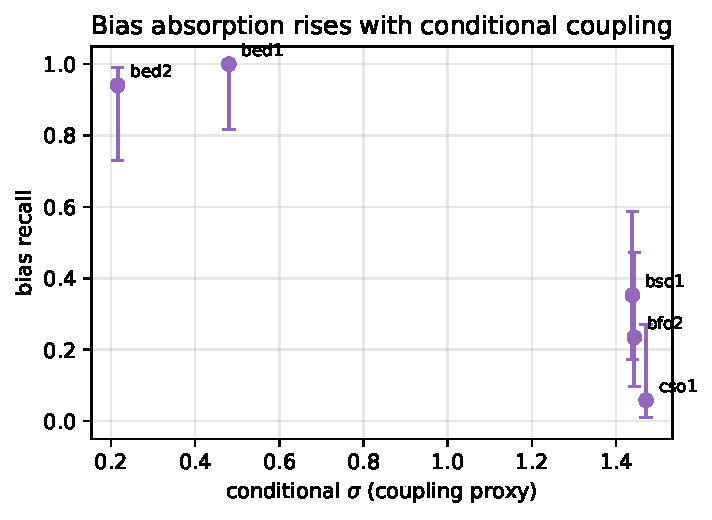
\includegraphics[width=0.8\linewidth]{figures/fig_bias_vs_sigma.pdf}
    \caption{Bias recall is monotone in conditional $\sigma$: a constant offset is isolated on weakly coupled (small-$\sigma$) channels and absorbed by the conditional mean on strongly coupled (large-$\sigma$) channels. Error bars are Wilson 95\% intervals. Source: \texttt{i7\_scaled\_bias\_by\_channel.csv}.}
    \label{fig:biascoupling}
\end{figure}

\subsection{Real bias and the detection floor}
\label{sec:lbnl}
The bias--coupling relationship above predicts that a constant offset is isolable only when it is large relative to the conditional scale of the signal it perturbs. We confirm this on a real labelled-fault dataset: the LBNL building-FDD MZVAV-1 set~\citep{LBNL_FDD2019,Granderson2023}, in which a constant offset of $\pm 1$, $\pm 2$, or $\pm 4\,^\circ$C is imposed on the outdoor-air-temperature sensor of a simulated multi-zone air-handling unit, with a per-timestamp fault label. We run the online adaptive detector over the four coupled AHU air temperatures (supply, outdoor, mixed, return), holding out the fault label, and measure typing on the biased outdoor-air-temperature signal (\texttt{i7\_lbnl\_bias.csv}).

The decisive quantity is the magnitude of the imposed bias in conditional-standard-deviation units. The outdoor-air-temperature conditional standard deviation on healthy data is $3.81\,^\circ$F, so the imposed offsets ($1.8$, $3.6$, $7.2\,^\circ$F) correspond to only $0.47$, $0.94$, and $1.89\,\sigma$ respectively---every one of them below the $3\sigma$ isolation threshold. The detector therefore correctly declines to flag them: detection of the biased signal is $0.27$--$0.33$ across the threshold sweep, and forcing detection upward by lowering the mean threshold to $2\sigma$ drives the healthy false-positive rate to $0.74$ (Table~\ref{tab:lbnl}). This is not a failure but a quantified \emph{detection floor}: a threshold-based typing layer isolates a bias only once it exceeds a few conditional standard deviations, by construction, and alarming below that floor would flood the operator with false positives. The result triangulates with the controlled study, whose injections at $4\sigma$ (above the floor) were isolable, and with the bias--coupling relationship: real sensor biases that are small relative to a signal's conditional scale are, and should be, below the alarm floor.

\begin{table}[t]
    \centering
    \caption{Real outdoor-air-temperature bias on LBNL MZVAV-1 (online adaptive detector). The imposed offsets are $0.47$--$1.89\,\sigma$, below the $3\sigma$ floor, so detection is low and cannot be raised without an unacceptable false-positive rate. Source: \texttt{i7\_lbnl\_bias.csv}.}
    \label{tab:lbnl}
    \begin{tabular}{rccc}
        \toprule
        Mean threshold & Healthy FP rate & Bias detection & Typed as bias \\
        \midrule
        2.0 & 0.743 & 0.332 & 0.034 \\
        3.0 & 0.686 & 0.302 & 0.018 \\
        4.0 & 0.657 & 0.280 & 0.009 \\
        5.0 & 0.634 & 0.269 & 0.006 \\
        \bottomrule
    \end{tabular}
\end{table}

\subsection{Freezing is type attribution, not detection capability}
\label{sec:freeze}
We initially expected freezing to be a detection blind spot of the base detector, on the reasoning that a signal stuck at a value within its normal range would not trigger a conditional-CDF alarm. This claim is refuted by our own validation. Table~\ref{tab:freeze} reports, per channel, the base CDF detection rate, the dedicated freeze-test detection rate, their median detection delays, and the fraction of trials in which the freeze test fired earlier (\texttt{i7\_freeze\_latency.csv}). The base CDF detector catches \emph{every} injected freeze on \emph{every} channel ($\texttt{cdf\_detect\_rate}=1.0$, $\texttt{frac\_cdf\_never}=0.00$ throughout), because the conditional expectation keeps moving while the frozen signal does not, driving the residual out of bounds. Moreover, the CDF detector is usually \emph{faster}: its median delay ranges from $2$ to $28$ steps, and the freeze test---whose fixed $25$-step confirmation window sets its median delay at exactly $25$---fires earlier in only about half the trials, and only on the most isolated channel (bed2, $\texttt{frac\_freeze\_earlier}=0.529$); on the most coupled channels it never beats the CDF detector ($0.0$).

\begin{table}[t]
    \centering
    \caption{Freezing detection: the base CDF detector catches every injected freeze on every channel, usually faster than the fixed $25$-step freeze test. Source: \texttt{i7\_freeze\_latency.csv} ($N=17$ per channel).}
    \label{tab:freeze}
    \begin{tabular}{lccccc}
        \toprule
        Channel & Cond.\ $\sigma$ & CDF detect & CDF median delay & Freeze earlier & CDF never \\
        \midrule
        bed2 & 0.216 & 1.0 & 28 & 0.529 & 0.0 \\
        bed1 & 0.480 & 1.0 & 9  & 0.294 & 0.0 \\
        bso1 & 1.439 & 1.0 & 17 & 0.412 & 0.0 \\
        bfo2 & 1.443 & 1.0 & 3  & 0.000 & 0.0 \\
        cso1 & 1.471 & 1.0 & 2  & 0.000 & 0.0 \\
        \bottomrule
    \end{tabular}
\end{table}

The conclusion is that the freeze test adds type \emph{attribution}---distinguishing a stuck sensor from a genuine process excursion---rather than detection capability or speed. The theoretical blind spot, in which the conditional standard deviation collapses to zero and the residual cannot grow, is an edge case that does not arise in the real or injected data we examined. On the real deployment this attribution is exactly what types the battery-depletion faults as freezing (Section~\ref{sec:operating-curve}), turning a detection into a maintenance label.

\subsection{Regime robustness comes from suppression, not residual cancellation}
\label{sec:regime}
We also expected the conditional residual to cancel coordinated shifts---a fault arriving as a shared shift across correlated signals would, on this reasoning, leave the conditional residual unchanged and so produce no spurious type label, independent of the change-point suppression. This claim is also refuted: residual cancellation (mechanism~1) is strongly correlation-dependent, and the robustness of the composed system instead comes from graded change-point suppression (mechanism~2). Table~\ref{tab:regime} reports the false-label rate across correlation $\rho$, coordinated-shift magnitude, and suppression scale (\texttt{i7\_regime\_fp.csv}, $5$ seeds per cell). With suppression disabled ($\texttt{scale}=1$), a $\geq 6\sigma$ coordinated shift at low correlation ($\rho=0.1$) produces about $20\%$ false labels ($0.199$ at $6\sigma$, $0.201$ at $10\sigma$); the boundary recedes as $\rho$ increases and is gone by $\rho \geq 0.7$. By contrast, the default graded suppression ($\texttt{scale}=5$) drives the false-label rate to exactly $0.0$ in every $(\rho, \text{shift})$ cell, as does full suppression ($\texttt{scale}=\infty$).

\begin{table}[t]
    \centering
    \caption{False-label rate under coordinated shifts co-occurring with a change point, by correlation $\rho$, shift magnitude, and suppression scale (mean over $5$ seeds). Residual cancellation alone ($\texttt{scale}=1$) fails at low correlation; graded suppression ($\texttt{scale}=5$) yields $0.0$ everywhere. Source: \texttt{i7\_regime\_fp.csv}.}
    \label{tab:regime}
    \begin{tabular}{ccccc}
        \toprule
        $\rho$ & Shift ($\sigma$) & \texttt{scale}=1 & \texttt{scale}=5 & \texttt{scale}=$\infty$ \\
        \midrule
        0.1 & 3  & 0.000 & 0.000 & 0.000 \\
        0.1 & 6  & 0.199 & 0.000 & 0.000 \\
        0.1 & 10 & 0.201 & 0.000 & 0.000 \\
        0.3 & 3  & 0.000 & 0.000 & 0.000 \\
        0.3 & 6  & 0.021 & 0.000 & 0.000 \\
        0.3 & 10 & 0.198 & 0.000 & 0.000 \\
        0.5 & 3  & 0.000 & 0.000 & 0.000 \\
        0.5 & 6  & 0.000 & 0.000 & 0.000 \\
        0.5 & 10 & 0.112 & 0.000 & 0.000 \\
        0.7 & 3--10 & 0.000 & 0.000 & 0.000 \\
        0.9 & 3--10 & 0.000 & 0.000 & 0.000 \\
        \bottomrule
    \end{tabular}
\end{table}

The adapt-into-drift robustness of the composed system therefore rests on mechanism~2, the graded change-point suppression, and not on the conditional-residual cancellation we originally credited. This matters operationally: the suppression scale is the parameter the operator must set, and it has a measurable cost, quantified next.

\begin{figure}[t]
    \centering
    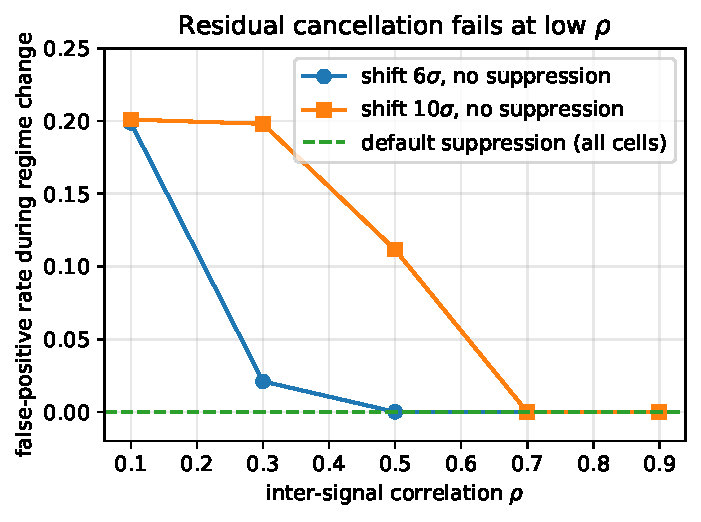
\includegraphics[width=0.8\linewidth]{figures/fig_regime_fp.pdf}
    \caption{Without change-point suppression, conditional-residual cancellation (mechanism~1) fails at low correlation: a large coordinated shift produces false fault labels until $\rho$ is high. The default graded suppression (mechanism~2) drives the rate to zero in every cell. Source: \texttt{i7\_regime\_fp.csv}.}
    \label{fig:regime}
\end{figure}

\subsection{The cost of suppression: dead-band and freeze-on-quiescent ablations}
\label{sec:ablation}
Suppression suppresses real faults too. Table~\ref{tab:deadband} reports the detection of a genuine drift that co-occurs with a change point, as a function of suppression scale (\texttt{i7\_deadband.csv}, $5$ seeds). With no suppression ($\texttt{scale}=1$) the drift is detected once it reaches $5.2\sigma$; at the default $\texttt{scale}=5$ detection is delayed until $17.6\sigma$; at $\texttt{scale}=\infty$ the drift is never detected. The default suppression thus opens a masking dead-band of roughly $[3\sigma, 15\sigma]$ for faults that happen to coincide with a change point---the measured price of the robustness reported in Section~\ref{sec:regime}.

\begin{table}[t]
    \centering
    \caption{Co-occurring-fault dead-band: detection magnitude of a drift co-occurring with a change point, by suppression scale ($5$ seeds). Source: \texttt{i7\_deadband.csv}.}
    \label{tab:deadband}
    \begin{tabular}{lccc}
        \toprule
        Suppression scale & Detected & Median delay & Magnitude at detection ($\sigma$) \\
        \midrule
        1.0      & yes & 26 & 5.2  \\
        5.0      & yes & 88 & 17.6 \\
        $\infty$ & no  & -- & --   \\
        \bottomrule
    \end{tabular}
\end{table}

\begin{figure}[t]
    \centering
    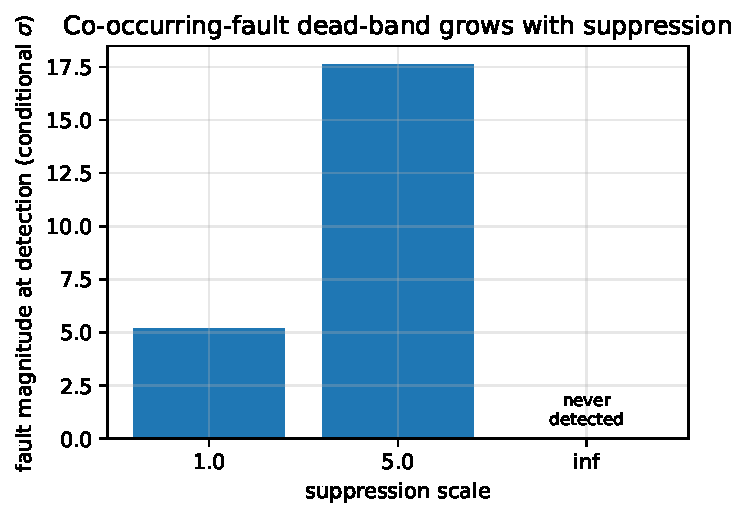
\includegraphics[width=0.7\linewidth]{figures/fig_deadband.pdf}
    \caption{The co-occurring-fault dead-band: a drift co-occurring with a change point must grow from $5.2\sigma$ (no suppression) to $17.6\sigma$ (default suppression) before detection, and is never detected under full suppression. Source: \texttt{i7\_deadband.csv}.}
    \label{fig:deadband}
\end{figure}

The freeze test similarly requires calibration on steady-state signals. Table~\ref{tab:quiescent} reports the false freeze-label rate on a genuinely live but very quiet signal (noise at $0.5\%$ of the marginal standard deviation) under three freeze-constant settings (\texttt{i7\_freeze\_quiescent.csv}, $5$ seeds). With the default constants, such a signal is falsely labelled frozen $72\%$ of the time; the loose constants make it worse ($\approx 88\%$); the strict constants ($\texttt{freeze\_eps}=10^{-4}$, $\texttt{freeze\_var\_ratio}=5\times10^{-3}$, $\texttt{freeze\_abs\_scale}=5$) eliminate the false label entirely ($0.0$). We therefore recommend the strict constants, or per-signal calibration, for deployments containing steady-state signals.

\begin{table}[t]
    \centering
    \caption{Freeze-on-quiescent ablation: false freeze-label rate on a live but quiet signal (noise $0.5\%$ of marginal std), by freeze-constant setting ($5$ seeds). Source: \texttt{i7\_freeze\_quiescent.csv}.}
    \label{tab:quiescent}
    \begin{tabular}{lccc}
        \toprule
        Freeze constants & \texttt{freeze\_eps} & \texttt{freeze\_var\_ratio} / \texttt{freeze\_abs\_scale} & False freeze rate \\
        \midrule
        default & $1\times10^{-3}$ & $1\times10^{-2}$ / $20$ & 0.717 \\
        loose   & $5\times10^{-3}$ & $5\times10^{-2}$ / $50$ & 0.887 \\
        strict  & $1\times10^{-4}$ & $5\times10^{-3}$ / $5$  & 0.000 \\
        \bottomrule
    \end{tabular}
\end{table}

\subsection{Detection baseline}
\label{sec:baseline}
Because the typing layer is only as useful as the detector beneath it, we confirm that the base detector is competitive with a published streaming alternative. Table~\ref{tab:baseline} compares it against the streaming autoencoder detector of \citet{Reunanen2020}---a one-pass, no-window outlier detector---under identical online point-wise evaluation on the SKAB multivariate benchmark ($37\,222$ points, $35.4\%$ anomalous; \texttt{i5\_reunanen\_skab.csv}). The base conditional-Gaussian detector outperforms the baseline on both threshold-free ROC AUC ($0.562$ vs $0.499$) and best-case F1 ($0.452$ vs $0.414$). Absolute values are modest because SKAB's anomalies are collective events that point-wise scoring penalises for any memory-less one-pass detector; the comparison is a relative positioning of the detector our typing layer extends, not a state-of-the-art detection claim.

\begin{table}[t]
    \centering
    \caption{Detection head-to-head on SKAB, identical online point-wise evaluation. Source: \texttt{i5\_reunanen\_skab.csv}.}
    \label{tab:baseline}
    \begin{tabular}{lcc}
        \toprule
        Detector & ROC AUC & Best F1 \\
        \midrule
        Base (conditional Gaussian) & \textbf{0.562} & \textbf{0.452} \\
        \citet{Reunanen2020} (streaming autoencoder) & 0.499 & 0.414 \\
        \bottomrule
    \end{tabular}
\end{table}

\subsection{Benchmark positioning on TSB-AD}
\label{sec:tsbad}
The SKAB head-to-head fixes the detector's position against one streaming alternative; we now place it on a large, public, multi-domain benchmark. We evaluate on the univariate split of TSB-AD \citep{Liu2024TSBAD} (350 evaluation series spanning 23 source domains), under the strict one-pass \emph{predict-then-learn} regime: every point is scored before the model is allowed to learn from it, so no future information leaks into any score. Hyperparameters for the base detector and the \citet{Reunanen2020} baseline are tuned on the official disjoint tuning split by Bayesian optimisation with an identical budget; the z-score and random detectors are the standard reference floors. We report VUS-PR, the metric the TSB-AD authors identify as the most reliable for ranking detectors (\texttt{tsb\_ad\_fullrun.csv}).

Table~\ref{tab:tsbad} shows the base detector leads on mean VUS-PR ($0.335$ vs $0.271$ for the z-score, $0.164$ for \citet{Reunanen2020}, and $0.092$ for the random floor). The result is not driven by a few easy series: in paired per-series comparison the detector beats the z-score on $83\%$ of the 350 series, \citet{Reunanen2020} on $87\%$, and the random floor on $89\%$, and it is the single best method on $17$ of the $23$ source domains. The mean exceeds the median ($0.174$) because a minority of well-separated domains (e.g.\ Exathlon $0.80$, NEK $0.63$, YAHOO $0.59$) score highly while a long tail of hard point-anomaly domains (notably UCR, where every method scores below $0.03$) pulls the centre down. The z-score edges the detector on a handful of domains dominated by sharp, isolated spikes (MITDB, SMAP, Stock, TAO), where a memory-less point statistic is hard to beat; these are exactly the regimes least relevant to the slow sensor faults the typing layer targets. The headline, then, is that a constant-memory, one-pass detector with online adaptation is competitive with---and on average ahead of---a tuned streaming baseline across a broad public benchmark, which is the foundation the typing layer requires.

\begin{table}[t]
    \centering
    \caption{TSB-AD univariate split (350 series), strict one-pass predict-then-learn, VUS-PR. ``AID win'' is the fraction of series on which the base detector scores higher than the row method. Source: \texttt{tsb\_ad\_fullrun.csv}.}
    \label{tab:tsbad}
    \begin{tabular}{lccc}
        \toprule
        Method & Mean VUS-PR (95\% CI) & Median & AID win \\
        \midrule
        Base detector (AID) & \textbf{0.335} [0.299, 0.371] & \textbf{0.174} & --- \\
        z-score & 0.271 [0.240, 0.302] & 0.148 & 83\% \\
        \citet{Reunanen2020} & 0.164 [0.139, 0.188] & 0.069 & 87\% \\
        Random & 0.092 [0.074, 0.109] & 0.039 & 89\% \\
        \bottomrule
    \end{tabular}
\end{table}

\begin{figure}[t]
    \centering
    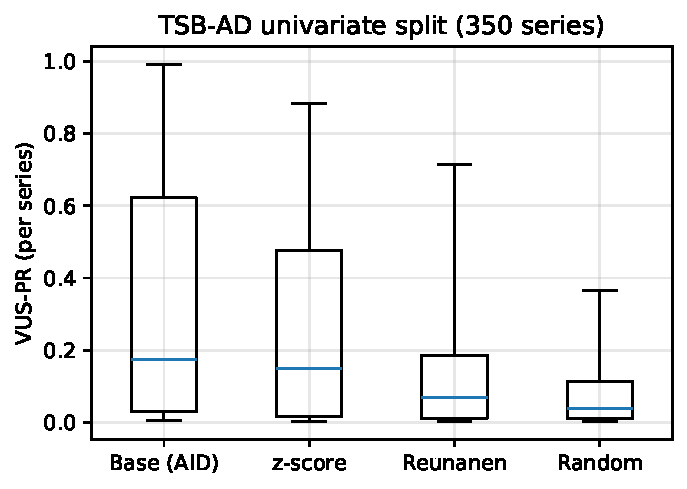
\includegraphics[width=0.7\linewidth]{figures/fig_tsbad_vuspr.pdf}
    \caption{Per-series VUS-PR distribution on the TSB-AD univariate split (350 series). Boxes span the interquartile range, whiskers the $5$th--$95$th percentiles; the base detector dominates both the median and the upper tail. Source: \texttt{tsb\_ad\_fullrun.csv}.}
    \label{fig:tsbad}
\end{figure}


\section{Discussion}
\label{Discussion}
The characterization in Section~\ref{Results} maps the operating envelope of the composed system honestly. We read each apparent limitation as a quantified property that an operator can plan around, rather than a defect to be hidden.

\paragraph{Bias absorption is a property of the interpretable model, not a bug.}
The monotone dependence of bias recall on conditional standard deviation (Table~\ref{tab:biascoupling}) follows directly from what makes the base detector interpretable. Because the conditional mean of a strongly coupled signal tracks its peers, a constant offset injected on that signal is partly explained away by the conditional model, and the residual---hence the typing---does not see it. The same mechanism that yields tight, peer-informed operating limits also absorbs offsets on those signals. The practical reading is that bias is reliably typed where it is observable (weakly coupled signals show recall up to $0.941$) and is absorbed where the model is confident enough to overrule it; the aggregate $0.518$ is the average of these two regimes, not a uniform failure. An operator who needs bias coverage on a strongly coupled signal should monitor that signal's raw calibration directly, a check the conditional model is, by construction, not designed to provide.

\paragraph{Two-signal cancellation limits the real-deployment false-positive floor.}
On the Intel Lab stream the residual healthy false positives are $\approx 93\%$ drift, traced to diurnal ramps that a two-signal conditional model cannot fully cancel. This is the same correlation-dependence quantified in Table~\ref{tab:regime}: with few correlated signals, slow shared movement leaks into the residual. The limitation is therefore structural and predictable---it improves with the number of correlated signals available---rather than a tuning failure. We report the $7.4\%$ floor at $90\%$ detection as the achievable operating point on a two-signal deployment, with the explicit expectation that richer instrumentation would lower it.

\paragraph{The dead-band is the priced cost of adaptation robustness.}
Because robustness to faults arriving during adaptation comes from graded change-point suppression and not from residual cancellation (Section~\ref{sec:regime}), it carries a cost: the masking dead-band of roughly $[3\sigma, 15\sigma]$ for faults co-occurring with a change point (Table~\ref{tab:deadband}). We present this as an explicit trade-off governed by a single parameter, \texttt{suppress\_scale}. A deployment that fears spurious labels from coordinated shifts should keep the default suppression; one that fears missing a fault during a regime change should lower it, accepting the false-label rate of Table~\ref{tab:regime}. The point is that the trade-off is measured and tunable, not silent.

\paragraph{Threshold and freeze-constant calibration are deployment decisions.}
The operating-point sweep (Table~\ref{tab:operating}) and the freeze-on-quiescent ablation (Table~\ref{tab:quiescent}) both show that the system's behavior is set by a small number of interpretable constants. The mean threshold selects the false-alarm/detection trade-off; the freeze constants determine how aggressively a quiet signal is judged frozen, with the strict setting eliminating false freeze labels on a live-but-quiet signal that the default mislabels $72\%$ of the time. We recommend the strict freeze constants or per-signal calibration for steady-state signals, and we expose the threshold as the operator's primary control. These are calibration decisions with quantified consequences, not hidden defaults.

\paragraph{Data availability constrains the evaluation to triangulation.}
No public stream simultaneously labels all four fault types per signal and per timestep, which is why we combine controlled injection (per-type ground truth, but synthetic) with a real fault deployment (genuine faults, but a single physical failure mode with a held-out label). Neither alone would be conclusive: the injections could overstate performance on idealized faults, and the real deployment exercises mainly the freezing signature. Read together, the injections establish the per-type envelope and the refuted claims, while the real deployment confirms that the envelope holds on genuine faults at a usable operating point. We regard this triangulation as the appropriate evidentiary standard given the data that exist, and we flag the absence of a fully labelled multi-type stream as the principal external constraint on stronger claims.


\section{Conclusion}
\label{Conclusion}
We presented a streaming sensor-fault classifier that closes the detection-to-action gap of a self-supervised online anomaly detector~\citep{Wadinger2023} by attributing each flagged signal to a maintenance-relevant fault type---bias, drift, accuracy loss, or freezing---from the detector's own conditional residuals, in O(1) memory and with no history buffers. The fault taxonomy is the established one~\citep{Sharma2010,Ni2009}; the contribution is its streaming, conditional-residual realization composed directly with the detector, so that type attribution is available at the same latency and operational footprint as detection.

The headline result is practical. On real battery-depletion faults in the Intel Berkeley Lab deployment~\citep{IntelLab2004}, the composed system reaches $90\%$ real-fault detection at a $7.4\%$ healthy false-positive rate and types the detected faults predominantly as freezing ($0.93$), the correct maintenance diagnosis for a transmitter stuck at a degraded value. Online adaptation is shown to be mandatory: a static prefix model false-alarms at $0.97$ on the same diurnal stream.

Around this result we characterized the operating envelope rather than overstating it. Freezing and drift are recovered with recall $1.000$ and $0.741$ on controlled injections, while bias recall is monotone in conditional coupling---absorbed on strongly coupled signals and isolated on weakly coupled ones---so that the aggregate $0.518$ is the mean of two explained regimes. We reported two refuted claims as such: freezing is not a detection blind spot of the base detector (which catches every injected freeze, usually faster than the dedicated test, so the freeze test contributes type attribution rather than detection), and adaptation robustness arises from graded change-point suppression rather than from conditional-residual cancellation. The suppression carries a measured masking dead-band of roughly $[3\sigma, 15\sigma]$ for co-occurring faults, and the freeze test requires strict constants or per-signal calibration on steady-state signals.

We also positioned the underlying detector on a broad public benchmark: on the TSB-AD univariate split ($350$ series, $23$ domains) under strict one-pass predict-then-learn it leads on mean VUS-PR and wins the majority of series against a tuned streaming baseline and the standard floors, confirming that the layer is built on a competitive detector. The scope is correspondingly honest. The real-deployment evidence exercises principally the freezing signature, the two-signal conditional model sets a structural false-positive floor that richer instrumentation would lower, per-type ground truth is available only through injection because no public stream labels all four fault types per signal and per timestep, and the benchmark evidence is univariate---the multivariate split, where the per-row conditional-MVN cost is substantial, is left to future work. Within that scope, the system delivers a deployable typing layer that turns an adaptive detector's alarm into an actionable maintenance label, with an operating envelope that is mapped rather than assumed.


\section{Reproducibility}
\label{Reproducibility}
Every number, table, and figure in this paper is reproducible from a
single pinned revision of the public repository
\url{https://github.com/MarekWadinger/safeband}, the git
tag \texttt{i7-fault-typing-v1}. The exact software environment is
captured by the committed \texttt{uv.lock} (resolved for Python~3.12);
\texttt{uv sync} recreates it deterministically. No value reported here
is transcribed by hand from a transient run: each experiment script
writes a CSV artifact under \texttt{examples/benchmarks/}, every table
and figure caption names its source CSV, and the four figures are
rendered from those CSVs by a single script,
\texttt{publications/I7\_fault\_typing/make\_figures.py}. The
benchmark scripts are deterministic (fixed seed~42).

\paragraph{Data provenance.}
The controlled-injection carrier (CATS nominal block) and the SKAB
detection benchmark are committed in the repository under
\texttt{examples/data/}. The three real-fault datasets are obtained from
their original sources into \texttt{.temp/data/} (not redistributed):
Intel Berkeley Lab from \url{https://db.csail.mit.edu/labdata/data.txt.gz};
the LBNL building-FDD set from OEDI submission~910,
\texttt{doi:10.25984/1824861}; and the TSB-AD benchmark from the
TheDatumOrg/TSB-AD repository. Each script aborts with a clear message
if its dataset is absent.

\paragraph{Artifact map.}
Table~\ref{tab:repro} lists, for each committed CSV, the script that
produces it; the table and figure captions in Section~\ref{Results} name
the CSV each draws from, closing the loop from raw data to typeset
result.

\begin{table}[t]
    \centering
    \caption{Mapping from each result artifact (CSV) to the committed script that produces it, at tag \texttt{i7-fault-typing-v1}. Figures are rendered from these CSVs by \texttt{make\_figures.py}.}
    \label{tab:repro}
    \begin{tabular}{ll}
        \toprule
        Result CSV (\texttt{examples/benchmarks/}) & Generating script (\texttt{examples/}) \\
        \midrule
        \texttt{i7\_scaled\_per\_type.csv} & \texttt{08\_i7\_scaled\_validation.py} \\
        \texttt{i7\_scaled\_bias\_by\_channel.csv} & \texttt{08\_i7\_scaled\_validation.py} \\
        \texttt{i7\_scaled\_normal\_precision.csv} & \texttt{08\_i7\_scaled\_validation.py} \\
        \texttt{i7\_freeze\_latency.csv} & \texttt{09\_i7\_freeze\_latency.py} \\
        \texttt{i7\_regime\_fp.csv} & \texttt{10\_i7\_regime\_fp.py} \\
        \texttt{i7\_deadband.csv} & \texttt{11\_i7\_ablations.py} \\
        \texttt{i7\_freeze\_quiescent.csv} & \texttt{11\_i7\_ablations.py} \\
        \texttt{i7\_intel\_lab\_operating\_points.csv} & \texttt{12\_i7\_intel\_lab\_realfaults.py} \\
        \texttt{i7\_intel\_lab\_fault\_types.csv} & \texttt{12\_i7\_intel\_lab\_realfaults.py} \\
        \texttt{i7\_lbnl\_bias.csv} & \texttt{13\_i7\_lbnl\_bias.py} \\
        \texttt{i5\_reunanen\_skab.csv} & \texttt{14\_i5\_reunanen\_headtohead.py} \\
        \texttt{tsb\_ad\_fullrun.csv} & \texttt{06\_tsb\_ad\_fullrun.py} \\
        \bottomrule
    \end{tabular}
\end{table}

The full procedure---environment, data acquisition, per-artifact
commands, and figure rendering---is documented in
\texttt{publications/I7\_fault\_typing/REPRODUCE.md} at the same tag.


\section*{Additional information}
The classifier and all evaluation artifacts are openly accessible on GitHub at \url{https://github.com/MarekWadinger/safeband} (pinned at git tag \texttt{i7-fault-typing-v1}; see Section~\ref{Reproducibility}).

\section*{CRediT authorship contribution statement}
\textbf{Marek Wadinger:} Conceptualization; Data curation; Formal analysis; Investigation; Methodology; Software; Validation; Visualization; Writing - original draft; and Writing - review \& editing. \textbf{Michal Kvasnica:} Conceptualization; Funding acquisition; Project administration; Resources; Supervision; Validation.

\section*{Declaration of Competing Interest}
The authors declare that they have no known competing financial interests or personal relationships that could have appeared to influence the work reported in this paper.

\section*{Acknowledgements}
The authors gratefully acknowledge the contribution of the Slovak Research and Development Agency under the project APVV-20-0261. The authors gratefully acknowledge the contribution of the Scientific Grant Agency of the Slovak Republic under the grant 1/0490/23. This paper was funded by the European Union under Horizon Europe Grant Agreement number 101079342 (Fostering Opportunities Towards Slovak Excellence in Advanced Control for Smart Industries).

\bibliographystyle{elsarticle-harv}
\bibliography{main}

\end{document}

\endinput
